\section{Data Construction}\label{data_construct}

\begin{comment}

\begin{figure}[t]
    \centering
    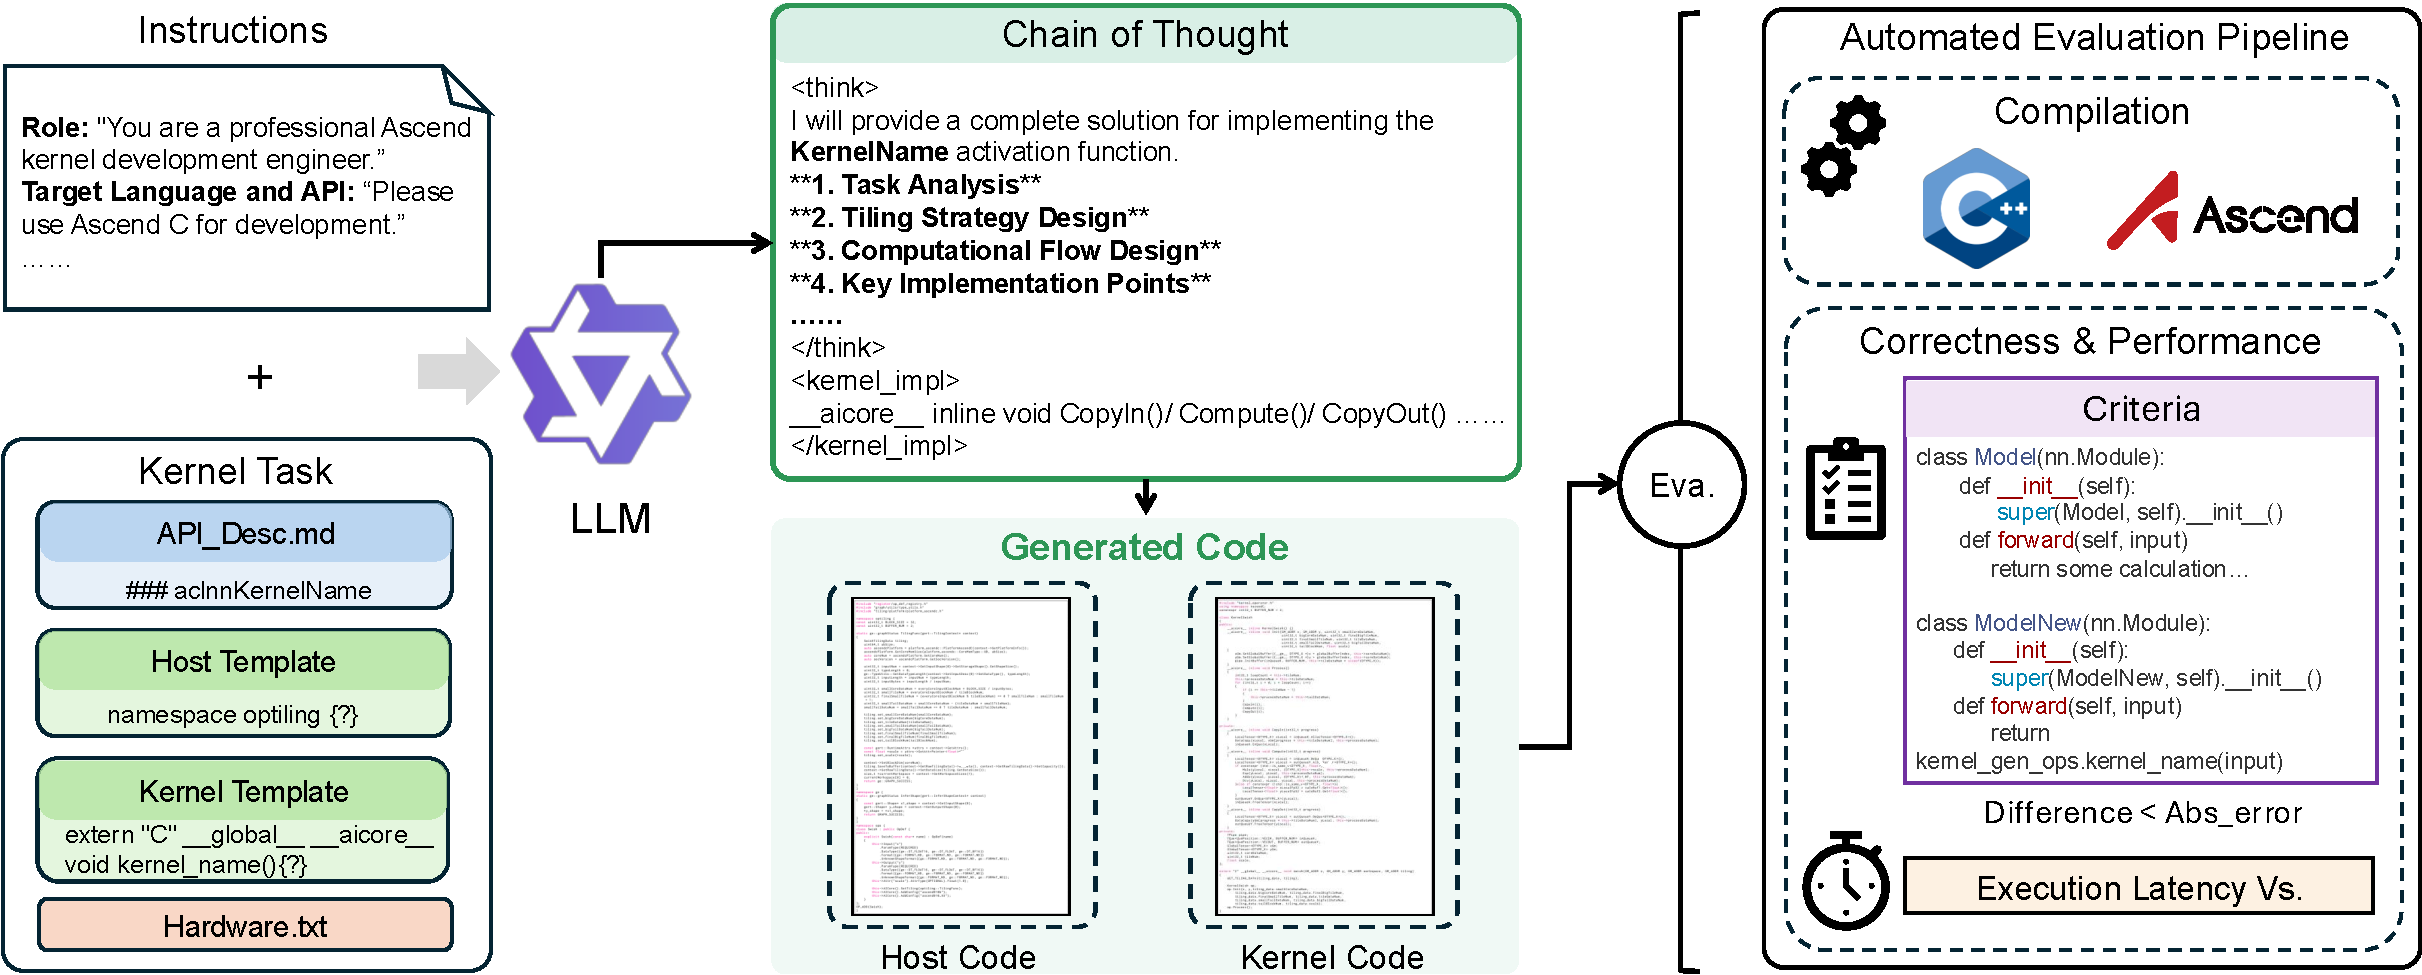
\includegraphics[width=1\linewidth]{pdfs/NPUKernelBench_Overview.pdf}
    \caption{Replace this with data construction figure.}
    \label{fig:Data_Constru}
\end{figure}

% To enable large language models (LLMs) to generate high-quality Huawei Ascend operators, we construct a multi-source dataset integrating both domain-specific and general reasoning data. Specifically, the dataset consists of three complementary components: (1) the \textbf{AscendC Developer Guide}, which provides authoritative and standardized documentation for custom operator development; (2) the \textbf{CANN Kernels}, containing real-world Ascend operator implementations at both single-file and project levels; and (3) the \textbf{General Reasoning Chains}, which includes 100K open-source reasoning traces from the DeepSeek-R1 corpus and high-quality C++ chain-of-thought data. The inclusion of general reasoning data prevents the model from overfitting to domain-specific syntax and ensures that it retains general reasoning and problem-solving abilities.
To enable large language models (LLMs) to generate high-quality Huawei Ascend operators, we construct a multi-source dataset that integrates domain-specific reasoning data with general reasoning data. Specifically, this dataset comprises three complementary components: (1) \textbf{AscendC Documentation Dataset}, which is constructed from official standardized custom operator development documentation to address the issue of models lacking domain knowledge of the Ascend; (2) \textbf{CANN Operator Code Dataset}, which is built from Huawei's open-source Ascend operator libraries (such as Ascend native operators in the MindSpore framework) and publicly available Ascend operator implementations from industry, to address the problem of models understanding functionality but being unable to write code; (3) \textbf{General Reasoning Chain}, which includes 100K open-source reasoning traces from the DeepSeek-R1 corpus and high-quality C++ chain-of-thought data. The inclusion of general reasoning data prevents the model from overfitting to domain-specific syntax and ensures that it retains general reasoning and problem-solving abilities.

\subsection{Ascend C Documentation Dataset}\label{document_dataset}
The Ascend C documentation contains comprehensive domain knowledge of Ascend, such as Ascend's hardware logic, language syntax, API usage, etc. To enable large language models to master the domain knowledge of Ascend C, we use the following three documents to construct the document data:

\textbf{(1) Ascend C Operator Development Guide.} This document introduces the fundamentals of operator development based on the Ascend C operator programming language, including abstract hardware architecture, programming models, etc. It covers both basic concepts for developers to quickly get started and in-depth analysis of core architecture and key technical principles to meet the needs of advanced users for deeper exploration.

\textbf{(2) Ascend C API Documentation.} This document provides a set of library APIs that enable developers to program using standard C++ syntax. The APIs are categorized into Kernel APIs for implementing operator kernel functions (including basic data structures like GlobalTensor and LocalTensor, basic APIs that abstract hardware capabilities, and high-level APIs that implement common computational algorithms), Host APIs (including Tiling APIs for high-level APIs, operator prototype registration and management APIs, Tiling data structure registration APIs, and platform information acquisition APIs), and operator debugging APIs for debugging and performance tuning.

\textbf{(3) Ascend C Best Practices.} This document presents performance optimization strategies, methods, and case studies for Ascend C operators, guiding developers to improve operator performance through an iterative optimization process that includes acquiring performance data, analyzing key performance bottlenecks, designing optimization solutions, and validating performance benefits.

To effectively inject domain knowledge into the model, we develop an automated pipeline that restructures documents into high-quality question-answer pairs with chains of thought reasoning. We adopt the Knowledge-Instruct framework to construct the document dataset in a fully automated manner. Unlike unsupervised continual pre-training (CPT) methods that directly feed entire documents into the base model, our knowledge injection approach significantly improves knowledge retention and mitigates the "hallucination" problem that occurs when small-parameter models learn large amounts of domain-specific knowledge.

\subsubsection{Basic Knowledge QA Data}
To enable large language models to understand domain knowledge of Ascend C, we construct high-quality CoT question-answering data using knowledge documents. Specifically, we first use large language models to generate questions from documents, then employ the RAG paradigm to construct high-quality chains of thought and answers, and perform data augmentation through paraphrasing.

\textbf{(1) Question Generation.} We first segment the documents and use large language models to convert them into JSON format files. Then we use large language models to generate multiple questions for each chapter and section, ensuring that every knowledge point in the document is covered by at least one question. In prompt design, we require the model to ask questions from different cognitive levels, focusing on technical details such as formulas, code, and API usage, while explicitly constraining to avoid duplicate questions and cross-framework content. We also record chapter numbers for subsequent use.

\textbf{(2) Relevant Chapter Retrieval.} We design chapter retrieval prompts to guide the model in locating relevant chapters from the document structure. The prompt follows a "fine-grained priority principle", requiring the model to prioritize selecting the deepest-level and most specific sub-chapters, avoiding the selection of coarse-grained chapters based solely on keyword matching. The model outputs the retrieved chapter IDs along with reasoning for the selection. Based on the retrieved chapter IDs, we load the corresponding document content and concatenate it to form a context-relevant complete prompt. For samples where retrieval fails, we adopt a fallback strategy, directly using the golden chapters recorded during question generation to supplement the context.

\textbf{(3) Chain of Thought and Answer Generation.} We design structured chain of thought generation prompts, requiring the model to output structured content containing both the chain of thought and answer sections. To ensure answer quality, the prompt explicitly prohibits the use of meta-task description terms such as "document", "reference content", and "prompt", making the generated content more natural and fluent. Additionally, we add a paraphrasing step to generate multiple differently-phrased question-answer pairs for the same knowledge point.

\subsubsection{API Call QA Data}
To enable large language models to learn how to call Ascend C API interfaces, we construct high-quality API question-answer pairs with chain-of-thought reasoning using API documentation. Specifically, we first crawl and fix the API documentation from official webpages, then automatically generate high-quality technical question-answer pairs that include a "thinking process" using large language models.

\textbf{(1) Documentation Crawling and Fixing.} To construct high-quality training data, we first need to obtain complete and accurate API documentation. However, the official online documentation presents two major challenges: mathematical formulas are displayed as images and content is scattered across multiple pages. To address this, we developed an intelligent scraping and repair tool that integrates three core technologies: web crawling, OCR recognition, and large language model semantic correction.

The entire process adopts a four-stage pipeline architecture: First, we use Selenium to launch a Headless Chrome browser and parse the documentation entry page to build an API link index. Then, we scrape HTML content page by page and extract plain text context. Next, for formula images in the documentation, we use OpenCV for preprocessing (scaling and binarization to enhance clarity), followed by the pix2tex engine to convert them into preliminary LaTeX code. Finally, we input both the OCR results and page context into the large language model, leveraging its semantic understanding capabilities to fix recognition errors (such as variable name confusion and hallucinated characters). The corrected LaTeX code is inserted into the HTML in \$...\$ format to replace the original image tags, and ultimately converted to Markdown format via markdownify and stored by API category. Through this end-to-end automated process, we successfully converted online documentation containing numerous formula images into high-quality Markdown documents in plain text format, establishing a solid foundation for subsequent question-answer pair generation.

\textbf{(2) Question-Answer Pair Generation.} Building upon the high-quality API documentation obtained after repair, we design an automated question-answer pair generation pipeline. The core of this pipeline leverages the reasoning capabilities of large language models, combined with carefully engineered prompts, to automatically extract and construct high-quality QA data with chain-of-thought reasoning from technical documentation.

For each API document, the system reads the complete content and constructs a structured prompt consisting of three core components: role definition, task constraints, and output format specifications. In prompt design, we emphasize five key requirements: first, the template-first principle, requiring at least one QA pair based on sample code from the documentation; second, complete context, ensuring questions contain all necessary code snippets to be self-contained; third, diversity coverage, asking questions from different dimensions such as parameters, overloads, and constraints; fourth, deep reasoning, requiring simulation of expert thinking processes within `<think>` blocks; fifth, traceability, attaching citations from the original text as evidence.

\subsection{AscendC Kernels}\label{kernel_dataset}
AscendC is a programming language introduced within the CANN Kit specifically for  kernel development scenarios. It follows standard C/C++ conventions and matches developers’ coding habits, while providing multi-layer interface abstractions, automatic parallelization, and twin-mode debugging to significantly improve kernel development efficiency. As part of Huawei’s heterogeneous computing stack, AscendC allows developers to fully exploit the parallel computing capabilities of Huawei’s Da Vinci–architecture NPUs (Neural Processing Units) and other AI-oriented hardware. Although NPUs were originally designed for accelerating deep learning workloads, the CANN software stack—through AscendC and interfaces such as AscendCL—enables developers to implement custom kernels and deploy AI models directly on the NPU with low overhead. This brings substantial acceleration across diverse AI-intensive tasks, including device-side intelligent inference, large-scale training, computer vision, and speech processing.

\begin{wraptable}{r}{0.54\textwidth}
\vspace{-10pt}
\centering
\begin{tcolorbox}[
    rounded corners,
    arc=3pt,
    enhanced,
    width=0.54\textwidth,
    colframe=codegreen, % <----- CHANGED
    colback=white,
    title=\textbf{An example of Kernel Code},
    fonttitle=\bfseries\small,
    boxrule=0.6pt,
    left=2pt,
    right=2pt,
    top=0pt,
    bottom=1pt
  ]
  
\begin{tcolorbox}[
      sharp corners,
      colframe=refgreen,
      colback=refgreen!5,
      colbacktitle=refgreen!15,
      coltitle=refgreen,
      boxrule=0.4pt,
      title={\textbf{Host}},
      fonttitle=\bfseries\small,
      left=0.5pt,
      right=0.5pt,
      top=-5pt,
      bottom=-5pt
    ]
\begin{lstlisting}[style=mystyle, frame=none,framerule=0pt, language=Python]
namespace optiling {
static ge::graphStatus TilingFunc(gert::TilingContext *context)
{ // Initialize tiling data structures and parameter configurations
    TilingData tiling;
    return ge::GRAPH_SUCCESS;
}
} // namespace optiling
namespace ops {
class AddCustom : public OpDef {
public:
    explicit AddCustom(const char *name) : OpDef(name)
    {// Define operator input/output types and computation configuration
    }
};
OP_ADD(AddCustom);
} // namespace ops
\end{lstlisting}
\end{tcolorbox}
\begin{tcolorbox}[
      sharp corners,
      colframe=refgreen,
      colback=refgreen!5,
      colbacktitle=refgreen!15,
      coltitle=refgreen,
      boxrule=0.4pt,
      title={\textbf{Kernel}},
      fonttitle=\bfseries\small,
      left=0.5pt,
      right=0.5pt,
      top=-5pt,
      bottom=-5pt
    ]
\begin{lstlisting}[style=mystyle, frame=none,framerule=0pt, language=Python]
class KernelAdd {
public:
    __aicore__ inline void Init(GM_ADDR x, GM_ADDR y, GM_ADDR z, uint32_t totalLength, uint32_t tileNum) { // Initialize global buffers and queues
    }
    __aicore__ inline void Process() {
        for (int32_t i = 0; i < loopCount; i++) {
            CopyIn(i);
            Compute(i);
            CopyOut(i);
        }
    }
private:
    __aicore__ inline void CopyIn(int32_t progress) {
    // Copy xGm and yGm to local tensors via inQueue
    }
    __aicore__ inline void Compute(int32_t progress) {
    // Dequeue xLocal, yLocal; perform Add; enqueue zLocal
        LocalTensor xLocal = inQueueX.DeQue<DTYPE_X>();
        LocalTensor yLocal = inQueueY.DeQue<DTYPE_Y>();
        LocalTensor zLocal = outQueueZ.AllocTensor<DTYPE_Z>();
        Add(zLocal, xLocal, yLocal, tileLength);
    }
    __aicore__ inline void CopyOut(int32_t progress) {
    // Copy zLocal back to zGm
    }
};
extern "C" __global__ __aicore__ void add_custom(GM_ADDR x, GM_ADDR y, GM_ADDR z) {
    KernelAdd op;
    op.Init(x, y, zzh);
    op.Process();
}
\end{lstlisting}
\end{tcolorbox}
\end{tcolorbox}
\vspace{-15pt}
\captionof{table}{AscendC kernel for vector addition.}
\label{tab:kernel_example}
\vspace{-30pt}
\end{wraptable}

To illustrate the structure of an AscendC operator, we present a complete vector-addition kernel example, shown in Table~\ref{tab:kernel_example}. This example reflects the standard design pattern of custom operators on Huawei Ascend NPUs, where the overall implementation is divided into two tightly coupled components: the \textit{Host-side Tiling implementation} and the \textit{Device-side Kernel implementation}. Together, these two components orchestrate data partitioning, memory transfer, and computation on the AI Core.

\textbf{(1) Host-side Tiling Implementation.}
Because the on-chip memory of Ascend AI Cores cannot store the full input and output tensors, the operator must process data in tiles. The process of partitioning large tensors into smaller chunks and determining how each tile is computed is referred to as \textit{tiling}. The tiling logic—also known as the \textit{tiling strategy} or \textit{Tiling Function}—calculates parameters such as the tile size, the number of iterations, and the memory layout.
Since these computations involve scalar operations and control logic rather than vectorized numerical computation, they are inefficient to execute on the AI Core. Therefore, AscendC places the tiling function on the host side (CPU), where the runtime prepares the tiling metadata and embeds it into a tiling structure that is passed to the device kernel.

\textbf{(2) Device-side Kernel Implementation.}
The device kernel integrates explicit \textit{memory management} and \textit{compute-intensive execution} on the AI Core. To handle the hierarchical memory architecture of Ascend NPUs, input tiles are staged from Global Memory (GM) to on-chip Local Memory (L1/L0) via \texttt{CopyIn()} using DMA queues, while \texttt{CopyOut()} writes results (\texttt{zLocal}) back to GM. This queue-based mechanism decouples data movement from computation, enabling pipelined overlap and high throughput. The core computation runs entirely on the AI Core: local tensors are dequeued (\texttt{inQueueX.DeQue()}, \texttt{inQueueY.DeQue()}), processed via the vectorized \texttt{Add()} intrinsic, and enqueued for output (\texttt{outQueueZ.EnQue()}). Guided by the host-provided tiling metadata, the kernel repeatedly executes this \texttt{CopyIn} → \texttt{Compute} → \texttt{CopyOut} pipeline to complete the operator efficiently.

% \textbf{2) Memory Management.} The Ascend architecture separates \textit{Global Memory (GM)} and \textit{Local Memory (L1/L0)}. Developers must explicitly manage data movement between these memory hierarchies to ensure efficient execution.
% In this kernel, \texttt{CopyIn()} transfers input data (\texttt{xGm}, \texttt{yGm}) from GM to local tensors (\texttt{xLocal}, \texttt{yLocal}); \texttt{Compute()} performs the addition on local tensors; and \texttt{CopyOut()} writes the computed result (\texttt{zLocal}) back to GM.
% Data transfers are handled via DMA queues, enabling pipelined overlap between communication and computation.

% \textbf{3) Device (AI Core) Kernel.} The core computation runs on the AI Core, where the operator executes in a pipelined manner. The queue mechanism decouples data movement and computation to improve throughput. During each iteration, \texttt{inQueueX.DeQue()} and \texttt{inQueueY.DeQue()} fetch local tensors, \texttt{Add()} performs element-wise addition, and \texttt{outQueueZ.EnQue()} pushes results to the output queue for write-back.

The overall process includes: (1) the host computes the tiling strategy, determines tile sizes and loop counts, and allocates GM buffers; (2) the runtime launches the kernel on the AI Core, passing GM addresses and tiling metadata; (3) \texttt{Init()} sets up local buffers, queue descriptors, and other resources based on the tiling configuration; (4) \texttt{Process()} executes tile-wise pipelined computation, where \texttt{CopyIn} transfers input tiles from GM to Local Memory, \texttt{Compute} performs vectorized addition on local tensors (\texttt{inQueueX.DeQue()}, \texttt{inQueueY.DeQue()}, \texttt{Add()}), and \texttt{CopyOut} writes results back to GM (\texttt{outQueueZ.EnQue()}); and (5) the host retrieves the final results from GM for validation.

\subsubsection{Single-File CoT Construction}\label{single_file}
This section aims to enable the LLM to learn kernel grammar by constructing high-quality code chain-of-thought from a single kernel file that can be compiled without errors. To achieve this, we follow a three-step pipeline: we first generate questions based on the given kernel code, then construct well-structured question–answer (QA) pairs that serve as the basis for reasoning, and finally feed these QA pairs into the LLM to produce detailed chain-of-thought explanations that guide the generation of correct answer code. 

\textbf{(1) Generating Question.}
To generate a question for each kernel file, we first analyze the internal call relationships to identify all dependent files. Based on this analysis, we reorganize the target file together with its dependencies into a single, self-contained code snippet that can be compiled without errors. This consolidated snippet is then provided—along with its dependency code—as input to the LLM, together with the prompt specified in Table~\ref{tab:prompt_single_file_qa}, to guide the LLM in generating a question that accurately reflects the code’s functionality.

\begin{wraptable}{l}{0.5\textwidth}
\vspace{-20pt}
\centering
\begin{tcolorbox}[
    sharp corners,
      colframe=reforange,
      colback=reforange!5,
      colbacktitle=reforange!15,
      coltitle=reforange,
      boxrule=0.4pt,
      title={\textbf{Prompt for generating question}},
      fonttitle=\bfseries\small,
      left=0.5pt,
      right=0.5pt,
      top=0.5pt,
      bottom=0.5pt
]
{\small
You are an expert in AscendC programming for the Huawei Ascend processor. Based on the provided answer code, please generate a corresponding request for that code.

\textbf{Background:} 

I maintain an AscendC operator repository that contains many operators, and each operator consists of multiple code files. I am constructing a dataset to train an LLM that can assist in writing AscendC operators. Each file within an operator will serve as a single training sample. I already have the answer code for each sample, but I still need to generate the corresponding request. After I provide you with a piece of answer code, your task is to analyze the code, understand and summarize its purpose, and then generate a request such that the provided code naturally serves as a correct response to that request. The request should be high-level and concise rather than overly detailed.

Please output the request in the following format:

\verb|<request>REQUEST_TEXT</request>| 

Note: Output only the final request—no reasoning process.

\textbf{Requirements:}

1. The request must capture the core functionality and purpose of the code.

2. The request should be clear and concise, avoiding unnecessary complexity.

The answer code is provided below:

[ ... Kernel code ... ]

}
\end{tcolorbox}
% \begin{tcolorbox}[
%     sharp corners,
%       colframe=reforange,
%       colback=reforange!5,
%       colbacktitle=reforange!15,
%       coltitle=reforange,
%       boxrule=0.4pt,
%       title={\textbf{Generated question samples}},
%       fonttitle=\bfseries\small,
%       left=0.5pt,
%       right=0.5pt,
%       top=0.5pt,
%       bottom=0.5pt
% ]
% {\small
% <request> Please create an interface header file for the Sigmoid operator that includes the required header references, uses the AscendC namespace, and provides a deprecation notice pointing to the new sigmoid.h file. </request>

% <request> Please implement an AscendC operator header file that defines the computation interface for the Swish activation function. The activation is defined as swish$(x) = x / (1 + e^{(-βx)})$, and it should support both half and float data types. </request>
% }
% \end{tcolorbox}
\vspace{-15pt}
\captionof{table}{Prompt for generating question.}
\label{tab:prompt_single_file_qa}
\vspace{-100pt}
\end{wraptable}



Examples of the generated questions include:

\noindent\parbox{\linewidth}{
\small
\texttt{<request> Please create an interface header file for the Sigmoid operator that includes the required header references, uses the AscendC namespace, and provides a deprecation notice pointing to the new sigmoid.h file. </request>}
}
\parbox{\linewidth}{
\small
\texttt{<request> Please implement an AscendC operator header file that defines the computation interface for the Swish activation function. The activation is defined as swish$(x) = x / (1 + e^{(-βx)})$, and it should support both half and float data types. </request>}
}

\textbf{(2) Constructing Standard QA Pairs.} Building on the questions generated in Step (1), we then construct standard question–answer (QA) pairs to guide the LLM and facilitate chain-of-thought (CoT) reasoning. Each QA pair corresponds to a single self-contained code snippet. In particular, the question includes both (i) the question describing the intended functionality and (ii) all necessary dependency code that the answer must incorporate. The answer then provides the complete implementation of the requested functionality.
By jointly packaging the request and its relevant dependencies into the question and pairing them with the correct implementation, we form high-quality training samples that precisely reflect the mapping from problem statements to valid code solutions. Examples of these QA pairs are provided in the Appendix.

\textbf{(3) Generating Code-centric CoT.}
After constructing the QA pairs, we feed the constructed QA pairs into the LLM to generate kernel-centric CoT reasoning. Each QA pair produces a corresponding reasoning trace, which is further organized into a unified JSON format for downstream use. Through this pipeline, we obtain over 7k high-quality kernel-centric CoT samples, forming a substantial and diverse dataset for supervised training. A full example of the generated CoT is provided in Table \ref{tab:singel_example} the Appendix.


\subsubsection{Project-level CoT Construction}\label{project_file}
This section aims to enable the LLM to generate a complete kernel. To achieve this goal, we first need to construct high-quality Chain-of-Thought (CoT) documents from Ascend C kernel source code, test cases, and hardware specifications, which guide Host-side tiling parameter computation and Kernel-side pipeline design, and are later verified and optimized. However, industrial-grade Ascend C operators are typically large composite files with numerous shape branches, data types, and hardware-specific logic, resulting in low signal-to-noise ratios and often exceeding the context window of large models. To address this difficulty, we develop an intelligent deconstruction pipeline that breaks down a complex composite operator into multiple clean Host-Kernel code pairs and automatically generates the corresponding API documentation. Based on this foundation, the overall workflow proceeds as follows: (1) decomposing the composite operator into logically pure one-to-one Host-Kernel pairs; (2) constructing prompts by integrating kernel code, test cases, and hardware configurations; (3) feeding the combined prompt into the LLM to generate kernel-centric CoT; and (4) verifying and selecting high-quality CoT files according to execution results.

\textbf{(1) Host-Kernel Decomposition.}
Industrial-grade AscendC kernels are typically composite structures that embed multiple Shapes, Dtypes, and hardware modes within deeply nested templates and conditional branches. Such complexity results in low signal-to-noise ratios and makes the code unsuitable as direct input for LLM. To address this, we design a Host–Kernel collaborative decomposition pipeline:
\begin{itemize}
    \item Kernel-side extraction. All mutually exclusive execution paths (e.g., float16, float32, int8) are identified and extracted into independent, logically pure Kernel fragments. Each fragment is associated with a unique tiling key representing the conditions that trigger its execution.
    \item Host-side pruning. Using the tiling key, only the Host-side branches required to generate that key are retained, producing a streamlined Host fragment that aligns precisely with the corresponding Kernel logic.
    \item Atomic sample construction. Each data scenario is thereby decomposed into a pair of noise-free Host–Kernel atomic samples, providing clean and contextually consistent inputs for CoT generation and model training.
\end{itemize}
Table \ref{tab:kernel_host_decompos} compares the operator structure before and after decoupling. After decoupling, each data scenario is mapped to its own isolated and self-contained Host–Kernel code pair.
\begin{table}[t]
\begin{tcolorbox}[
sharp corners,
      colframe=refgreen,
      colback=refgreen!5,
      colbacktitle=refgreen!15,
      coltitle=refgreen,
      boxrule=0.4pt,
      title={\textbf{Host-Kernel Decomposition}},
      fonttitle=\bfseries\small,
      top=-10pt, bottom=0pt, left=1pt, right=1pt
]
\begin{tabular}{p{0.48\textwidth} p{0.48\textwidth}}
\begin{lstlisting}[basicstyle=\ttfamily\scriptsize]
# Before decomposing
.../{op_name}/answer/
+-- 0/
    |-- op_host/
    |   |-- add_custom.h
    |   `-- add_custom.cpp
    `-- op_kernel/
        |-- add_custom.h
        `-- add_custom.cpp
\end{lstlisting}
&
\begin{lstlisting}[basicstyle=\ttfamily\scriptsize]
# After decomposing
.../{op_name}/answer/
+-- 0/
|   +-- ... (Original backup)
+-- 1/
|   +-- op_host/ (<- The Host code of scenario 1.)
|   |   +-- add_custom.h
|   |   `-- add_custom.cpp
|   +-- op_kernel/
|   |   +-- add_custom.h
|   |   `-- add_custom.cpp
|   `-- tiling_key.json
`-- 2/
    +-- op_host/ (<- The Host code of scenario 2.)
    |   +-- add_custom.h
    |   `-- add_custom.cpp
    +-- op_kernel/
    |   +-- add_custom.h
    |   `-- add_custom.cpp
    `-- tiling_key.json
\end{lstlisting}
\end{tabular}
\end{tcolorbox}
\caption{The kernel code structure before and after decoupling. }
\label{tab:kernel_host_decompos}
\end{table}

\textbf{(2) Constructing Prompt.}
To effectively guide the LLM in generating a complete kernel project, it is necessary to construct CoT at the project level for supervised finetuning. Consequently, prior to formulating the CoT, we first design the prompt that will serve as its structural basis. In particular, the prompt is composed of four elements: the instruction text, kernel source code, test cases, and NPU hardware configuration. These components are then concatenated in a predefined order, thereby forming a single, coherent input file that is subsequently provided to the model. The full prompt specification is presented in Table~\ref{tab:prompt_project_file} in the Appendix.


\textbf{(3) Generating Kernel-centric CoT.}
After constructing the prompt, we feed it to the LLM to generate the kernel-centric CoT. In particular, the “thinking” component encompasses both the design of host-side tiling strategies and the implementation and pipeline design on the kernel side. Moreover, we also output a JSON summary containing all tiling parameter values following the generated thought chain. This summary is subsequently used to evaluate the quality of the CoT in the following sections. The generated CoT example is presented in Table~\ref{tab:prompt_project_file} in the Appendix.

\textbf{(4) CoT Verification and Optimization.}
To ensure high-quality CoTs, we perform two sequential steps:
\textbf{(a) Verification.} We first verify correctness by comparing the tiling JSON generated in Step (3) against predefined Gold Standard Logs, thereby validating the accuracy of the inferred tiling parameters.
\textbf{(b) Optimization.} Since the initial CoTs contain substantial redundant summarization that obscures core reasoning, we then refine only those CoTs that pass verification. Specifically, We automatically simplify their content to remove redundancy and highlight the essential tiling and pipelined reasoning steps. This is achieved using a tailored System Prompt that defines the LLM as a CoT optimization expert, together with a User Prompt specifying the optimization goals and modification rules. The complete prompts are provided in Table~\ref{tab:optimization_prompt}. This two-stage process ensures that the final CoTs are both reliable and well structured for subsequent evaluations.



\subsection{General Reasoning Chains}
% At the mean time, we also 

% Integrating explicit domain knowledge, whether through structured prompting or targeted fine-tuning, can significantly enhance the capability of LLMs in domain-specific code generation, including specialized tasks such as kernel development.
Leveraging the CoT datasets constructed in Sec.~\ref{kernel_dataset} and Sec.~\ref{document_dataset}, we fine-tune the LLM to better handle domain-specific kernel generation. However, relying exclusively on kernel-oriented data risks catastrophic forgetting. To balance specialization and generality, we incorporate several open-source CoT datasets~\cite{Chinese-Data-Distill-From-R1,AM-DeepSeek-R1-0528-Distilled,r1-dataset-collection-2025,reasoning_gemini_300k_2025}, including Chinese-Deepseek-R1-Distill-data-110k, AM-deepseek-R1-0528-Distilled, math-code-science-deepseek-r1-en, and reasoning\_gemini\_300k.

To ensure high-quality and consistent supervision across heterogeneous sources, we apply a unified cleaning pipeline with the following steps:

\textbf{(1) Language filtering and normalization.}
\begin{itemize}
    \item We remove samples written in low-resource languages, convert Traditional Chinese to Simplified Chinese, and enforce language ratios specific to each type of data: 5\% Chinese / 95\% English for code-related samples, and 50\% Chinese / 50\% English for math-related or code–math hybrid samples.
\end{itemize}


\textbf{(2) Task-specific filtering.}
\begin{itemize}
    \item Code-related samples: retain only samples with code length greater than 2k tokens and perplexity (if available) below 3.5;
    \item Math-related or code–math hybrid samples: retain only samples longer than 1.5k tokens with perplexity (if available) below 3.5.
\end{itemize}
This pipeline ensures that the resulting dataset is clean, balanced, and suitable for both general reasoning and domain-specific code or math tasks.

% To ensure data quality, we further perform a thorough cleaning process.
% First, we filter out CoT samples written in low-resource languages.
% Second, for code-related data, we retain only samples whose code length exceeds 2 and whose perplexity (when available) is below 3.5. We convert Traditional Chinese to Simplified Chinese and maintain an overall ratio of 5\% Chinese to 95\% English.
% Finally, for code-related data, we keep samples longer than 1.5k tokens with perplexity (if available) below 3.5, ensuring a 50\%-Chinese / 50\%-English balance.

% \subsubsection{Open-Source CoT Dataset}



% \subsubsection{high-quality C++ Cot Samples}

\end{comment}

%\begin{comment}

To equip large language models (LLMs) with the reasoning capabilities required for low-level NPU kernel generation, we construct a multi-source dataset that integrates domain-specific kernel knowledge with general reasoning supervision. The design goal is not only to expose the model to the surface form of AscendC kernels, but also to teach how expert developers reason about tiling strategies, memory movement, API constraints, and correctness under hardware-specific execution models.

As illustrated in Fig.~\ref{fig:framework}, the dataset consists of three complementary components: documentation-based reasoning data derived from AscendC manuals, kernel-centric chain-of-thought (CoT) data extracted from real-world AscendC operators, and general reasoning chains to preserve generalization capability. In total, the raw corpus contains 83,916 samples and is publicly available at \href{https://huggingface.co/AscendKernelGen/datasets}{\textcolor{blue}{Ascend-CoT}}.

The raw dataset exhibits a long-tailed length distribution. Approximately 99.1\% of samples have input sequences shorter than 11.1k tokens, although the maximum input length reaches about 111k tokens. On the output side, 85.1\% of samples are within 21.9k tokens and an additional 6.3\% fall between 21.9k and 43.8k tokens, while the maximum output length reaches about 219k tokens. Before supervised fine-tuning, we apply length-aware preprocessing: samples exceeding 32k tokens are discarded, and short samples are packed into fixed-length training sequences using boundary-aware isolation to prevent interference across concatenated examples. After preprocessing, the final SFT corpus consists of 9,955 sequences of length 32k.

\subsection{Documentation-Based CoT Data}
\label{document_dataset}

The AscendC programming ecosystem contains rich but highly specialized knowledge spanning hardware abstractions, programming models, and low-level API semantics. To inject this domain knowledge into LLMs in a controllable manner, we transform official AscendC documentation into structured, reasoning-oriented supervision rather than treating it as unstructured text.

Specifically, we construct documentation-based supervision from three authoritative sources: the AscendC Operator Development Guide, which introduces hardware abstractions and the programming model; the AscendC API Reference, which specifies kernel, host, and debugging interfaces; and the AscendC Best Practices, which describe performance optimization strategies and common pitfalls. Together, these sources provide comprehensive coverage of both functional correctness and performance-oriented considerations.

Instead of unsupervised continual pre-training, we adopt a \emph{knowledge-instruct} paradigm that converts documentation content into question–-answer pairs augmented with explicit reasoning traces. The resulting supervision emphasizes not only factual knowledge of APIs and concepts, but also the reasoning process underlying correct API usage and constraint satisfaction. This design mitigates hallucination caused by shallow pattern memorization and encourages systematic reasoning about hardware and programming constraints.

The constructed documentation-based dataset covers both conceptual reasoning over hardware abstractions and programming semantics, as well as API-centric reasoning that focuses on invocation patterns, parameter constraints, and typical error scenarios. Each sample consists of a natural-language question, a structured chain of reasoning, and a grounded answer. To ensure coverage and diversity, we enforce fine-grained chapter alignment and apply paraphrase augmentation during data generation.

\begin{comment}

\paragraph{Basic Knowledge and API Reasoning QA.}
From the documentation, we automatically construct two types of supervision:
\begin{itemize}
    \item Conceptual reasoning QA, which focuses on hardware concepts, programming models, and execution semantics;
    \item API-centric reasoning QA, which teaches correct API invocation patterns, parameter constraints, and typical error scenarios.
\end{itemize}

Each sample contains a natural-language question, a structured chain of reasoning, and a grounded answer. To ensure coverage and diversity, we enforce fine-grained chapter alignment and paraphrase augmentation during generation.

\end{comment}

\subsection{Code-Centric CoT Data}
\label{kernel_dataset}

Beyond documentation, correct kernel generation requires understanding how host-side tiling logic interacts with device-side kernel execution in practice. To capture this interaction, we construct code-centric chain-of-thought (CoT) data from real-world AscendC operator implementations.

For standalone kernel files that can be compiled independently, we generate kernel-level CoT samples that explicitly explain kernel structure, memory movement, and computation logic. Each sample pairs a functional specification with a complete kernel implementation and an explicit reasoning trace that justifies key design decisions, such as tiling assumptions, buffer usage, and pipeline organization.

However, industrial-grade AscendC operators are typically implemented as composite projects that support multiple shapes, data types, and execution branches. These implementations interleave host-side tiling logic with device-side kernel invocation, making them unsuitable for direct supervision. To address this challenge, we systematically decompose complex operators into logically pure host--kernel pairs, where each pair corresponds to a single execution scenario with fixed tiling and shape assumptions.

For each decomposed host--kernel pair, we construct project-level CoT supervision that jointly reasons about host-side tiling parameter computation, kernel-side pipeline structure and memory staging, and the consistency between tiling metadata and kernel execution behavior. This joint reasoning explicitly exposes the cross-boundary dependencies that are essential for correct kernel generation but are rarely visible in isolated kernel code.

To ensure correctness and executability, we retain only CoT samples that pass automated verification against reference tiling configurations. This filtering step guarantees that the generated reasoning traces are not only conceptually coherent but also aligned with valid host--kernel execution semantics.

\begin{comment}

\paragraph{Single-File Kernel Reasoning.}
For standalone kernel files that compile independently, we generate code-centric CoT samples that explain kernel structure, memory movement, and computation logic. Each sample pairs a functional specification with a complete implementation and an explicit reasoning trace that justifies design decisions.

\paragraph{Project-Level Kernel Reasoning.}
Industrial-grade AscendC operators are often implemented as large composite projects with multiple shapes, data types, and execution branches, making them unsuitable for direct supervision. To address this, we decompose complex operators into logically pure host–kernel pairs, each corresponding to a single execution scenario.

For each decomposed Host--Kernel pair, we construct project-level CoT supervision that jointly reasons about host-side tiling parameter computation, kernel-side pipeline structure and memory staging, as well as the consistency between tiling metadata and kernel execution.

Only CoT samples that pass automated verification against reference tiling configurations are retained, ensuring that the reasoning traces are both correct and executable.

\end{comment}

\subsection{General CoT Data}
\label{general_cot}

While domain-specific supervision is essential, training exclusively on kernel data risks degrading general reasoning ability. To balance specialization and generality, we augment our dataset with high-quality open-source chain-of-thought corpora covering mathematics, code reasoning, and scientific problem solving~\cite{Chinese-Data-Distill-From-R1,AM-DeepSeek-R1-0528-Distilled,r1-dataset-collection-2025,reasoning_gemini_300k_2025}.

We apply a unified filtering and normalization pipeline to ensure consistency across heterogeneous sources, including language normalization, length-based filtering, and perplexity-based quality control. This mixture allows the model to retain general problem-solving skills while adapting to the highly specialized reasoning demands of NPU kernel generation.

%\end{comment}